\documentclass[11pt,a4paper]{article}

% ---------- packages ----------
\usepackage[utf8]{inputenc}
\usepackage[T1]{fontenc}
\usepackage{lmodern}           % Latin Modern fonts
\usepackage{microtype}
\usepackage[margin=2.5cm]{geometry}
\usepackage{graphicx}
\usepackage{xcolor}
\usepackage{booktabs}
\usepackage{longtable}
\usepackage{amsmath,amssymb}
\usepackage{hyperref}
\usepackage{fancyhdr}
\usepackage{titlesec}
\usepackage{tcolorbox}
\usepackage{listings}
\usepackage{enumitem}
\usepackage{float}
\usepackage{caption}
\usepackage{subcaption}
\usepackage{multicol}

% ---------- colors ----------
\definecolor{accent}{HTML}{3898EC}
\definecolor{accentdark}{HTML}{140D44}
\definecolor{coral}{HTML}{D97757}
\definecolor{teal}{HTML}{4EC9B0}
\definecolor{codebg}{HTML}{F5F5F5}
\definecolor{codefg}{HTML}{2D2D2D}
\definecolor{codekey}{HTML}{0077AA}
\definecolor{codestr}{HTML}{669900}
\definecolor{codecom}{HTML}{999999}

% ---------- hyperref ----------
\hypersetup{
    colorlinks=true,
    linkcolor=accentdark,
    urlcolor=accent,
    citecolor=coral,
    pdftitle={lagCAMB Manual},
    pdfauthor={lagCAMB},
}

% ---------- headers ----------
\pagestyle{fancy}
\fancyhf{}
\fancyhead[L]{\small\textcolor{accent}{\textbf{lagCAMB}} Manual}
\fancyhead[R]{\small\thepage}
\fancyfoot[C]{\small\textcolor{gray}{Beyond-$\Lambda$CDM Cosmology with CAMB}}
\renewcommand{\headrulewidth}{0.4pt}
\renewcommand{\footrulewidth}{0.2pt}

% ---------- section style ----------
\titleformat{\section}
  {\Large\bfseries\color{accentdark}}
  {\thesection}{1em}{}[\vspace{-0.5em}\textcolor{accent}{\rule{\textwidth}{0.5pt}}]
\titleformat{\subsection}
  {\large\bfseries\color{accentdark}}
  {\thesubsection}{1em}{}

% ---------- code style ----------
\lstdefinestyle{python}{
    language=Python,
    basicstyle=\small\ttfamily\color{codefg},
    keywordstyle=\color{codekey}\bfseries,
    stringstyle=\color{codestr},
    commentstyle=\color{codecom}\itshape,
    backgroundcolor=\color{codebg},
    frame=single,
    framerule=0.5pt,
    rulecolor=\color{accent!40},
    breaklines=true,
    showstringspaces=false,
    tabsize=4,
    xleftmargin=1em,
    xrightmargin=1em,
    aboveskip=0.8em,
    belowskip=0.5em,
    morekeywords={camb,CAMBparams,set_cosmology,set_params,
        get_results,get_cmb_power_spectra,set_for_lmax,
        DarkMatter,DarkEnergy,WantTransfer,set_matter_power,
        get_matter_power_spectrum,DMBaryonScattering,
        DMDR_ETHOS,DecayingDM,DMNeutrinoScattering,
        FuzzyDM,WarmDM,DMPhotonScattering,MultiInteractingDM,
        InteractingDE,HorndeskiDE,FuzzyDMField,MG},
}
\lstset{style=python}

% ---------- tcolorbox ----------
\newtcolorbox{parambox}[1]{
    colback=codebg,
    colframe=accent!60,
    fonttitle=\bfseries,
    title={#1},
    sharp corners,
    boxrule=0.5pt,
    left=6pt, right=6pt, top=4pt, bottom=4pt,
}

\newtcolorbox{notebox}{
    colback=coral!8,
    colframe=coral!60,
    fonttitle=\bfseries,
    title={Note},
    sharp corners,
    boxrule=0.5pt,
    left=6pt, right=6pt, top=4pt, bottom=4pt,
}

\newtcolorbox{physbox}[1]{
    colback=teal!5,
    colframe=teal!60,
    fonttitle=\bfseries,
    title={#1},
    sharp corners,
    boxrule=0.5pt,
    left=6pt, right=6pt, top=4pt, bottom=4pt,
}

% ---------- document ----------
\begin{document}

% ============================================================
% TITLE PAGE
% ============================================================
\begin{titlepage}
\centering
\vspace*{3cm}
{\Huge\bfseries\color{accentdark} lagCAMB\\[0.3em]}
{\LARGE\color{accent} Beyond-$\Lambda$CDM Models for CAMB}\\[2cm]
{\Large User Manual}\\[1cm]
\textcolor{gray}{\rule{0.6\textwidth}{0.5pt}}\\[1cm]
{\large
Dark Matter Interactions $\bullet$ Modified Gravity\\[0.3em]
Interacting Dark Energy $\bullet$ Ultralight Axions\\[0.3em]
Warm/Decaying Dark Matter}\\[2cm]
{\normalsize Version 1.0 --- \today}\\[0.5cm]
{\normalsize Based on CAMB (Code for Anisotropies in the Microwave Background)}\\[0.3cm]
{\small\textcolor{gray}{A. Lewis, A. Challinor \& A. Lasenby (2000)}}
\vfill
\end{titlepage}

\tableofcontents
\newpage

% ============================================================
\section{Introduction}
% ============================================================

\textbf{lagCAMB} extends the standard CAMB Boltzmann solver with a modular framework for beyond-$\Lambda$CDM physics. All new models are implemented as plug-in classes inheriting from \texttt{TDarkMatterModel} (dark matter sector) or \texttt{TDarkEnergyModel} (dark energy / modified gravity), with minimal modifications to the core solver.

\subsection{Quick Start}

All models follow the same pattern:

\begin{lstlisting}
import camb
from camb.dark_matter import DMBaryonScattering  # or any model

pars = camb.CAMBparams()
pars.set_cosmology(H0=67.5, ombh2=0.022, omch2=0.122)
pars.InitPower.set_params(As=2.1e-9, ns=0.965)
pars.set_for_lmax(2500, lens_potential_accuracy=1)

# Activate a dark matter model
pars.DarkMatter = DMBaryonScattering()
pars.DarkMatter.set_params(sigma_dmb=1e-41, n_dmb=0, m_dm=1.0)

results = camb.get_results(pars)
cls = results.get_cmb_power_spectra(CMB_unit='muK')['total']
\end{lstlisting}

\subsection{Cosmological Baseline}

Unless otherwise noted, all comparison plots use the following baseline cosmology:
\begin{center}
\begin{tabular}{lll}
\toprule
Parameter & Value & Description \\
\midrule
$H_0$ & 67.5 km/s/Mpc & Hubble constant \\
$\Omega_b h^2$ & 0.022 & Baryon density \\
$\Omega_c h^2$ & 0.122 & CDM density \\
$A_s$ & $2.1\times10^{-9}$ & Scalar amplitude \\
$n_s$ & 0.965 & Spectral index \\
$\ell_{\max}$ & 2500 & Multipole truncation \\
\bottomrule
\end{tabular}
\end{center}

\subsection{Model Summary}

\begin{center}
\small
\begin{tabular}{llll}
\toprule
\textbf{Model} & \textbf{Type} & \textbf{Primary Effect} & \textbf{Reference} \\
\midrule
DM--Baryon & DM & CDM--baryon drag & Boddy \& Gluscevic 2018 \\
DM--DR (ETHOS) & DM & DM--dark radiation coupling & Cyr-Racine+ 2016 \\
Decaying DM & DM & CDM decay to daughter + DR & Blackadder+ 2014 \\
DM--Neutrino & DM & CDM--neutrino scattering & He+ 2023 \\
Fuzzy DM & DM & Quantum Jeans suppression & Hu+ 2000 \\
Warm DM & DM & Free-streaming suppression & Viel+ 2005 \\
DM--Photon & DM & CDM--photon opacity & Boddy \& Gluscevic 2018 \\
Multi-IDM & DM & Combined channels & Becker+ 2021 \\
Interacting DE & DE & DM--DE energy exchange & Costa+ 2017 \\
Horndeski & DE/MG & Scalar-tensor gravity (QSA) & Bellini \& Sawicki 2014 \\
$\mu$-$\Sigma$ MG & MG & Phenomenological MG & Zhao+ 2009 \\
\bottomrule
\end{tabular}
\end{center}


% ============================================================
% DARK MATTER MODELS
% ============================================================
\newpage
\section{Dark Matter Models}

% -------- DM-Baryon --------
\subsection{DM--Baryon Scattering}

\begin{physbox}{Physics}
Dark matter scatters off baryons with a velocity-dependent momentum-transfer cross section:
\begin{equation}
    \sigma_{\rm MT} = \sigma_0 \left(\frac{v}{c}\right)^n
\end{equation}
where $n \in \{-4, -2, 0, 2, 4\}$. This adds a drag force between the CDM and baryon fluids, suppressing small-scale structure and modifying the CMB damping tail. The back-reaction on baryons is included via momentum conservation.
\end{physbox}

\begin{parambox}{Parameters}
\begin{tabular}{llll}
\toprule
Name & Type & Default & Description \\
\midrule
\texttt{sigma\_dmb} & float & 0.0 & Cross section $\sigma_0$ [cm$^2$] \\
\texttt{n\_dmb} & int & 0 & Velocity index ($-4,-2,0,2,4$) \\
\texttt{m\_dm} & float & 100.0 & DM particle mass [GeV] \\
\bottomrule
\end{tabular}
\end{parambox}

\begin{lstlisting}
from camb.dark_matter import DMBaryonScattering

pars = camb.CAMBparams()
pars.set_cosmology(H0=67.5, ombh2=0.022, omch2=0.122)
pars.InitPower.set_params(As=2.1e-9, ns=0.965)
pars.set_for_lmax(2500, lens_potential_accuracy=1)
pars.WantTransfer = True
pars.set_matter_power(redshifts=[0], kmax=10.0)

pars.DarkMatter = DMBaryonScattering()
pars.DarkMatter.set_params(sigma_dmb=1e-41, n_dmb=0, m_dm=1.0)
# n_dmb=0: constant cross section
# Lighter DM (m_dm=1 GeV) gives stronger effect

results = camb.get_results(pars)
\end{lstlisting}

\begin{figure}[H]
\centering
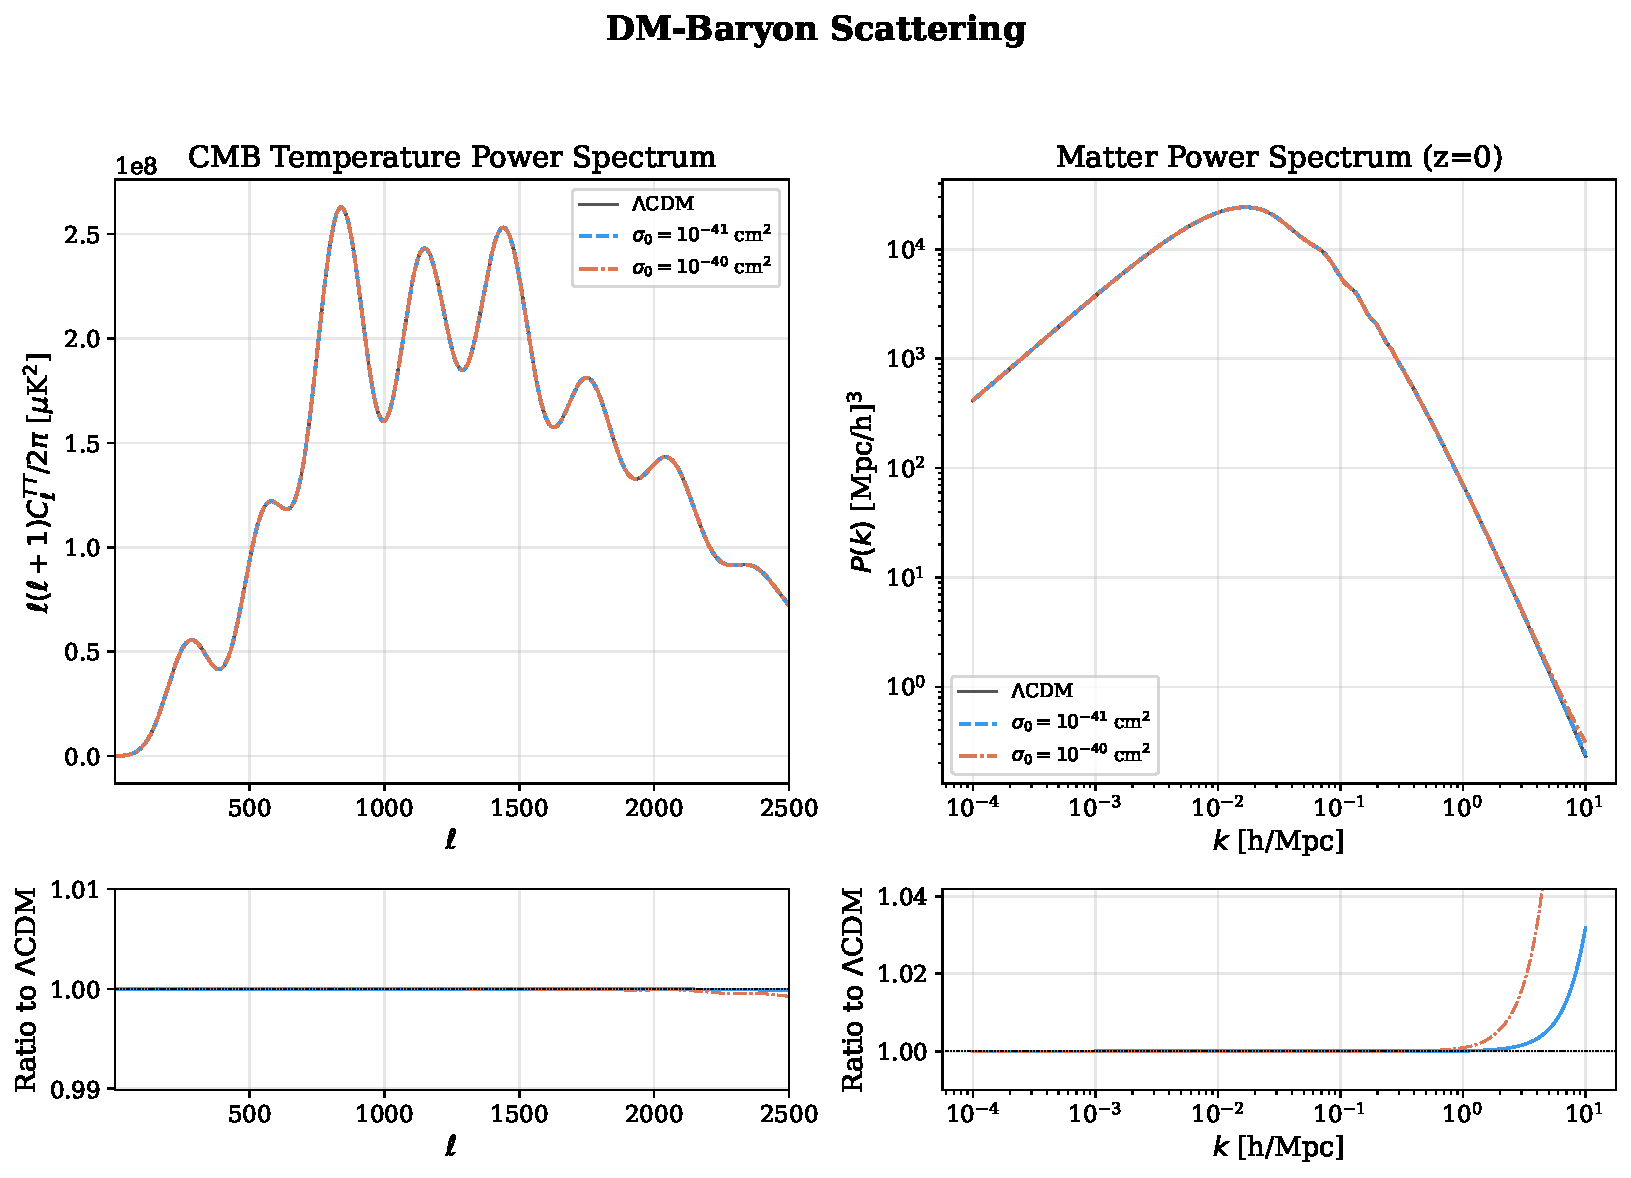
\includegraphics[width=\textwidth]{figures/dm_baryon_scattering.pdf}
\caption{DM--Baryon scattering: CMB TT power spectrum and matter power spectrum compared to $\Lambda$CDM. Parameters: $n=0$ (constant cross section), $m_{\rm DM}=1$ GeV.}
\end{figure}

\begin{notebox}
Drag rates are internally capped at $10^4 \times \dot{a}/a$ to prevent ODE stiffness at very early times. For $n_{\rm dmb} = -4$ (Coulomb-like), the effect is strongest at low velocities (late times).
\end{notebox}


% -------- DM-DR ETHOS --------
\newpage
\subsection{DM--Dark Radiation (ETHOS)}

\begin{physbox}{Physics}
In the ETHOS (Effective Theory of Structure Formation) framework, dark matter couples to a dark radiation sector via scattering. DM evolves as a fluid ($\delta_{\rm DM}$, $v_{\rm DM}$) while DR is described by a Boltzmann hierarchy ($F_0, F_1, \ldots, F_{\ell_{\max}}$). The opacity is parameterized as:
\begin{equation}
    \dot{\kappa} = \sum_{n=2}^{6} a_n \left(\frac{T_{\rm DR}}{T_0}\right)^n
\end{equation}
The interaction produces dark acoustic oscillations (DAO) analogous to baryon acoustic oscillations. Three regimes are automatically handled: tight coupling (TCA, $\Gamma \gg k$), full Boltzmann hierarchy, and ultra-relativistic fluid approximation (UFA, $k\tau \gg 1$).
\end{physbox}

\begin{parambox}{Parameters}
\begin{tabular}{llll}
\toprule
Name & Type & Default & Description \\
\midrule
\texttt{omdmdrh2} & float & 0.0 & Interacting DM density $\Omega_{\rm dmdr}h^2$ \\
\texttt{N\_dark} & float & 0.0 & DR effective number $\Delta N_{\rm eff}$ \\
\texttt{a\_dark} & list & None & ETHOS opacity coefficients $[a_2, \ldots, a_6]$ \\
\texttt{alpha\_l\_dark} & float & 1.0 & Angular damping for $\ell \ge 2$ \\
\texttt{lmax\_dr} & int & 15 & DR hierarchy truncation \\
\texttt{cs2\_dm} & float & 0.0 & DM sound speed squared \\
\bottomrule
\end{tabular}
\end{parambox}

\begin{lstlisting}
from camb.dark_matter import DMDR_ETHOS

pars = camb.CAMBparams()
pars.set_cosmology(H0=67.5, ombh2=0.022, omch2=0.122)
pars.InitPower.set_params(As=2.1e-9, ns=0.965)
pars.set_for_lmax(2500, lens_potential_accuracy=1)
pars.WantTransfer = True
pars.set_matter_power(redshifts=[0], kmax=10.0)

pars.DarkMatter = DMDR_ETHOS()
pars.DarkMatter.set_params(
    omdmdrh2=0.005,       # 5% of CDM is interacting
    N_dark=1.0,           # 1 DR species
    a_dark=[1e5],         # strong coupling
    lmax_dr=15            # Boltzmann hierarchy depth
)
results = camb.get_results(pars)
\end{lstlisting}

\begin{figure}[H]
\centering
\includegraphics[width=\textwidth]{figures/dm_dark_radiation_(ethos).pdf}
\caption{DM--DR (ETHOS): Dark acoustic oscillations appear in both CMB and $P(k)$ at scales entering the horizon before DM--DR decoupling. Stronger coupling ($a_{\rm dark} = 10^5$) produces deeper oscillations.}
\end{figure}

\begin{notebox}
The implementation uses a tight-coupling approximation (TCA) when the DM--DR interaction rate exceeds $50k$, eliminating stiff coupling terms from the ODE system. This allows stable integration even for very large $a_{\rm dark}$ values ($\sim 10^7$).
\end{notebox}


% -------- Decaying DM --------
\newpage
\subsection{Decaying Dark Matter}

\begin{physbox}{Physics}
A fraction $f_{\rm dcdm}$ of CDM decays into a massive daughter particle and dark radiation:
\begin{equation}
    \text{DM}_{\rm parent} \rightarrow \text{DM}_{\rm daughter}\;(\text{mass fraction } \epsilon) + \text{DR}
\end{equation}
The parent density evolves as $\rho_{\rm dcdm}(a) = \rho_0\, a^{-3}\, e^{-\Gamma t(a)}$. The daughter receives a velocity kick $v_{\rm kick} = (1-\epsilon^2)/(2\epsilon)$, and the DR is accumulated from decay products evolving via a truncated Boltzmann hierarchy.
\end{physbox}

\begin{parambox}{Parameters}
\begin{tabular}{llll}
\toprule
Name & Type & Default & Description \\
\midrule
\texttt{Gamma\_dcdm} & float & 0.0 & Decay rate [km/s/Mpc] \\
\texttt{epsilon\_dcdm} & float & 1.0 & $m_{\rm daughter}/m_{\rm parent}$ \\
\texttt{f\_dcdm} & float & 1.0 & Fraction of CDM that decays \\
\bottomrule
\end{tabular}
\end{parambox}

\begin{lstlisting}
from camb.dark_matter import DecayingDM

pars = camb.CAMBparams()
pars.set_cosmology(H0=67.5, ombh2=0.022, omch2=0.122)
pars.InitPower.set_params(As=2.1e-9, ns=0.965)
pars.set_for_lmax(2500, lens_potential_accuracy=1)
pars.WantTransfer = True
pars.set_matter_power(redshifts=[0], kmax=10.0)

pars.DarkMatter = DecayingDM()
pars.DarkMatter.set_params(
    Gamma_dcdm=100,       # decay rate ~ H_0
    epsilon_dcdm=0.9,     # 10% mass lost to DR per decay
    f_dcdm=0.1            # 10% of CDM decays
)
results = camb.get_results(pars)
\end{lstlisting}

\begin{figure}[H]
\centering
\includegraphics[width=\textwidth]{figures/decaying_dark_matter.pdf}
\caption{Decaying DM: Decay transfers CDM energy to relativistic DR, reducing matter density at late times. The daughter particle's velocity kick also contributes to small-scale suppression.}
\end{figure}

\begin{notebox}
The decay rate $\Gamma$ is in the same units as $H_0$ [km/s/Mpc]. $\Gamma \sim H_0 \approx 67.5$ means the decay lifetime is comparable to the age of the universe. $\epsilon = 1$ corresponds to no mass loss (no decay effect).
\end{notebox}


% -------- DM-Neutrino --------
\newpage
\subsection{DM--Neutrino Scattering}

\begin{physbox}{Physics}
Dark matter scatters off neutrinos with an energy-dependent cross section:
\begin{equation}
    \sigma = \sigma_0 \left(\frac{E_\nu}{1\;\text{MeV}}\right)^n
\end{equation}
This adds drag to the CDM velocity equation and collision damping to the neutrino Boltzmann hierarchy, coupling CDM to the neutrino free-streaming scale.
\end{physbox}

\begin{parambox}{Parameters}
\begin{tabular}{llll}
\toprule
Name & Type & Default & Description \\
\midrule
\texttt{sigma\_dmnu} & float & 0.0 & Cross section at $E_0=1$ MeV [cm$^2$] \\
\texttt{n\_dmnu} & int & 0 & Energy index (0 or 2) \\
\texttt{m\_dm} & float & 100.0 & DM mass [GeV] \\
\bottomrule
\end{tabular}
\end{parambox}

\begin{lstlisting}
from camb.dark_matter import DMNeutrinoScattering

pars = camb.CAMBparams()
pars.set_cosmology(H0=67.5, ombh2=0.022, omch2=0.122)
pars.InitPower.set_params(As=2.1e-9, ns=0.965)
pars.set_for_lmax(2500, lens_potential_accuracy=1)
pars.WantTransfer = True
pars.set_matter_power(redshifts=[0], kmax=10.0)

pars.DarkMatter = DMNeutrinoScattering()
pars.DarkMatter.set_params(
    sigma_dmnu=1e-33,     # cross section [cm^2]
    n_dmnu=0,             # constant cross section
    m_dm=0.1              # 100 MeV DM
)
results = camb.get_results(pars)
\end{lstlisting}

\begin{figure}[H]
\centering
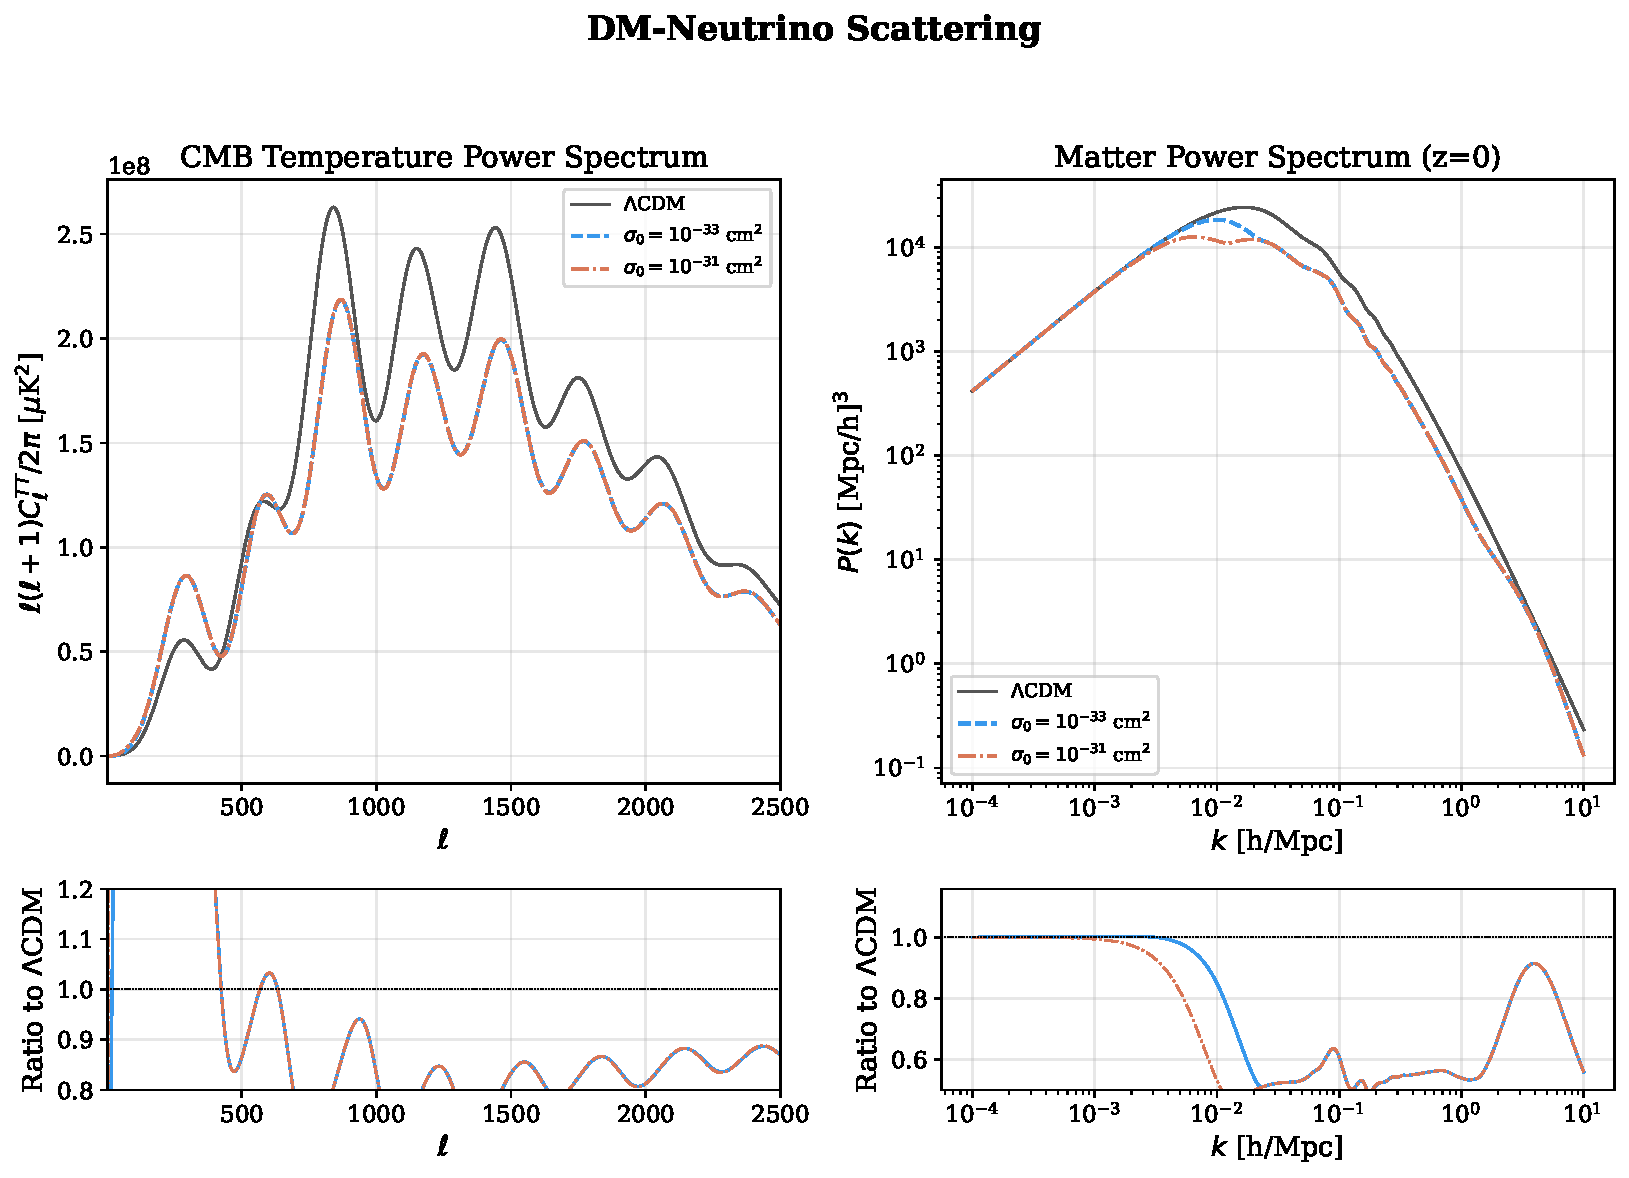
\includegraphics[width=\textwidth]{figures/dm_neutrino_scattering.pdf}
\caption{DM--Neutrino scattering: Coupling CDM to neutrinos delays matter domination on small scales and suppresses the matter power spectrum. Lighter DM gives a stronger per-particle scattering rate.}
\end{figure}


% -------- Fuzzy DM --------
\newpage
\subsection{Fuzzy Dark Matter}

\begin{physbox}{Physics}
Ultralight axion dark matter ($m \sim 10^{-22}$ eV) with de Broglie wavelength on astrophysical scales. The effective fluid has a scale-dependent sound speed:
\begin{equation}
    c_s^2(k, a) = \frac{k^2}{4\, m^2\, a^2}
\end{equation}
producing a quantum Jeans scale $k_J^2 = 4\, m_{\rm conf}\, a^2\, \dot{a}/a$ below which density perturbations are suppressed by quantum pressure.
\end{physbox}

\begin{parambox}{Parameters}
\begin{tabular}{llll}
\toprule
Name & Type & Default & Description \\
\midrule
\texttt{m\_axion} & float & $10^{-22}$ & Axion mass [eV] \\
\texttt{omega\_axion\_h2} & float & 0.0 & Axion density $\Omega_a h^2$ (0 uses \texttt{f\_axion}) \\
\texttt{f\_axion} & float & 1.0 & Fraction of CDM that is ULDM \\
\bottomrule
\end{tabular}
\end{parambox}

\begin{lstlisting}
from camb.dark_matter import FuzzyDM

pars = camb.CAMBparams()
pars.set_cosmology(H0=67.5, ombh2=0.022, omch2=0.122)
pars.InitPower.set_params(As=2.1e-9, ns=0.965)
pars.set_for_lmax(2500, lens_potential_accuracy=1)
pars.WantTransfer = True
pars.set_matter_power(redshifts=[0], kmax=10.0)

pars.DarkMatter = FuzzyDM()
pars.DarkMatter.set_params(
    m_axion=1e-24,        # 10^{-24} eV
    f_axion=0.3           # 30% of CDM is ULDM
)
results = camb.get_results(pars)
\end{lstlisting}

\begin{figure}[H]
\centering
\includegraphics[width=\textwidth]{figures/fuzzy_dark_matter.pdf}
\caption{Fuzzy DM: Quantum pressure suppresses $P(k)$ below the Jeans scale, with smaller masses producing suppression at larger scales. The CMB is affected through the integrated Sachs--Wolfe effect.}
\end{figure}

\begin{notebox}
A full Klein--Gordon field implementation (\texttt{FuzzyDMField}) is also available in the DarkEnergy slot, solving the exact background evolution including the frozen-field era and Passaglia--Hu improved EFA for perturbations. See Section~\ref{sec:fuzzyfield}.
\end{notebox}


% -------- Warm DM --------
\newpage
\subsection{Warm Dark Matter}

\begin{physbox}{Physics}
Thermal relic WDM with free-streaming that suppresses small-scale structure. In transfer-function mode (default):
\begin{equation}
    T(k) = \left[1 + (\alpha\, k)^{2\nu}\right]^{-5/\nu}
\end{equation}
where $\alpha$ depends on $m_{\rm WDM}$, $\Omega_{\rm WDM}$, and $h$. In Boltzmann mode, WDM is treated as an extra massive neutrino species using CAMB's full neutrino hierarchy.
\end{physbox}

\begin{parambox}{Parameters}
\begin{tabular}{llll}
\toprule
Name & Type & Default & Description \\
\midrule
\texttt{m\_wdm} & float & 3.0 & WDM mass [keV] \\
\texttt{T\_wdm\_ratio} & float & 1.0 & $T_{\rm WDM}/T_\nu$ ratio \\
\texttt{Omega\_wdm\_h2} & float & 0.0 & WDM density (0 = all CDM) \\
\texttt{boltzmann\_mode} & bool & False & Full Boltzmann vs transfer function \\
\bottomrule
\end{tabular}
\end{parambox}

\begin{lstlisting}
from camb.dark_matter import WarmDM

pars = camb.CAMBparams()
pars.set_cosmology(H0=67.5, ombh2=0.022, omch2=0.122)
pars.InitPower.set_params(As=2.1e-9, ns=0.965)
pars.set_for_lmax(2500, lens_potential_accuracy=1)
pars.WantTransfer = True
pars.set_matter_power(redshifts=[0], kmax=10.0)

pars.DarkMatter = WarmDM()
pars.DarkMatter.set_params(m_wdm=1.0)  # 1 keV WDM
results = camb.get_results(pars)
\end{lstlisting}

\begin{figure}[H]
\centering
\includegraphics[width=\textwidth]{figures/warm_dark_matter.pdf}
\caption{Warm DM: Free-streaming suppresses $P(k)$ at scales below the free-streaming horizon. Lighter particles ($m=1$ keV) produce stronger suppression at larger scales.}
\end{figure}

\begin{notebox}
In transfer-function mode (default), the CMB power spectrum is unchanged from $\Lambda$CDM. Only the matter power spectrum is modified via the transfer function. Set \texttt{boltzmann\_mode=True} to include CMB effects via the full Boltzmann hierarchy.
\end{notebox}


% -------- DM-Photon --------
\newpage
\subsection{DM--Photon Scattering}

\begin{physbox}{Physics}
DM scatters off photons with a temperature-dependent cross section:
\begin{equation}
    \sigma = \sigma_{\rm Th}\; u_{\rm idm\text{-}g}\; \frac{m_{\rm DM}}{100\;\text{GeV}} \left(\frac{T}{T_0}\right)^{n_{\rm idm\text{-}g}}
\end{equation}
This adds opacity to the photon hierarchy (extra scattering beyond Thomson) and drag to the CDM velocity.
\end{physbox}

\begin{parambox}{Parameters}
\begin{tabular}{llll}
\toprule
Name & Type & Default & Description \\
\midrule
\texttt{u\_idm\_g} & float & 0.0 & Dimensionless coupling \\
\texttt{n\_idm\_g} & int & 0 & Temperature power index \\
\texttt{m\_dm} & float & 100.0 & DM mass [GeV] \\
\bottomrule
\end{tabular}
\end{parambox}

\begin{lstlisting}
from camb.dark_matter import DMPhotonScattering

pars = camb.CAMBparams()
pars.set_cosmology(H0=67.5, ombh2=0.022, omch2=0.122)
pars.InitPower.set_params(As=2.1e-9, ns=0.965)
pars.set_for_lmax(2500, lens_potential_accuracy=1)
pars.WantTransfer = True
pars.set_matter_power(redshifts=[0], kmax=10.0)

pars.DarkMatter = DMPhotonScattering()
pars.DarkMatter.set_params(u_idm_g=1e-4, n_idm_g=0, m_dm=100.)
results = camb.get_results(pars)
\end{lstlisting}

\begin{figure}[H]
\centering
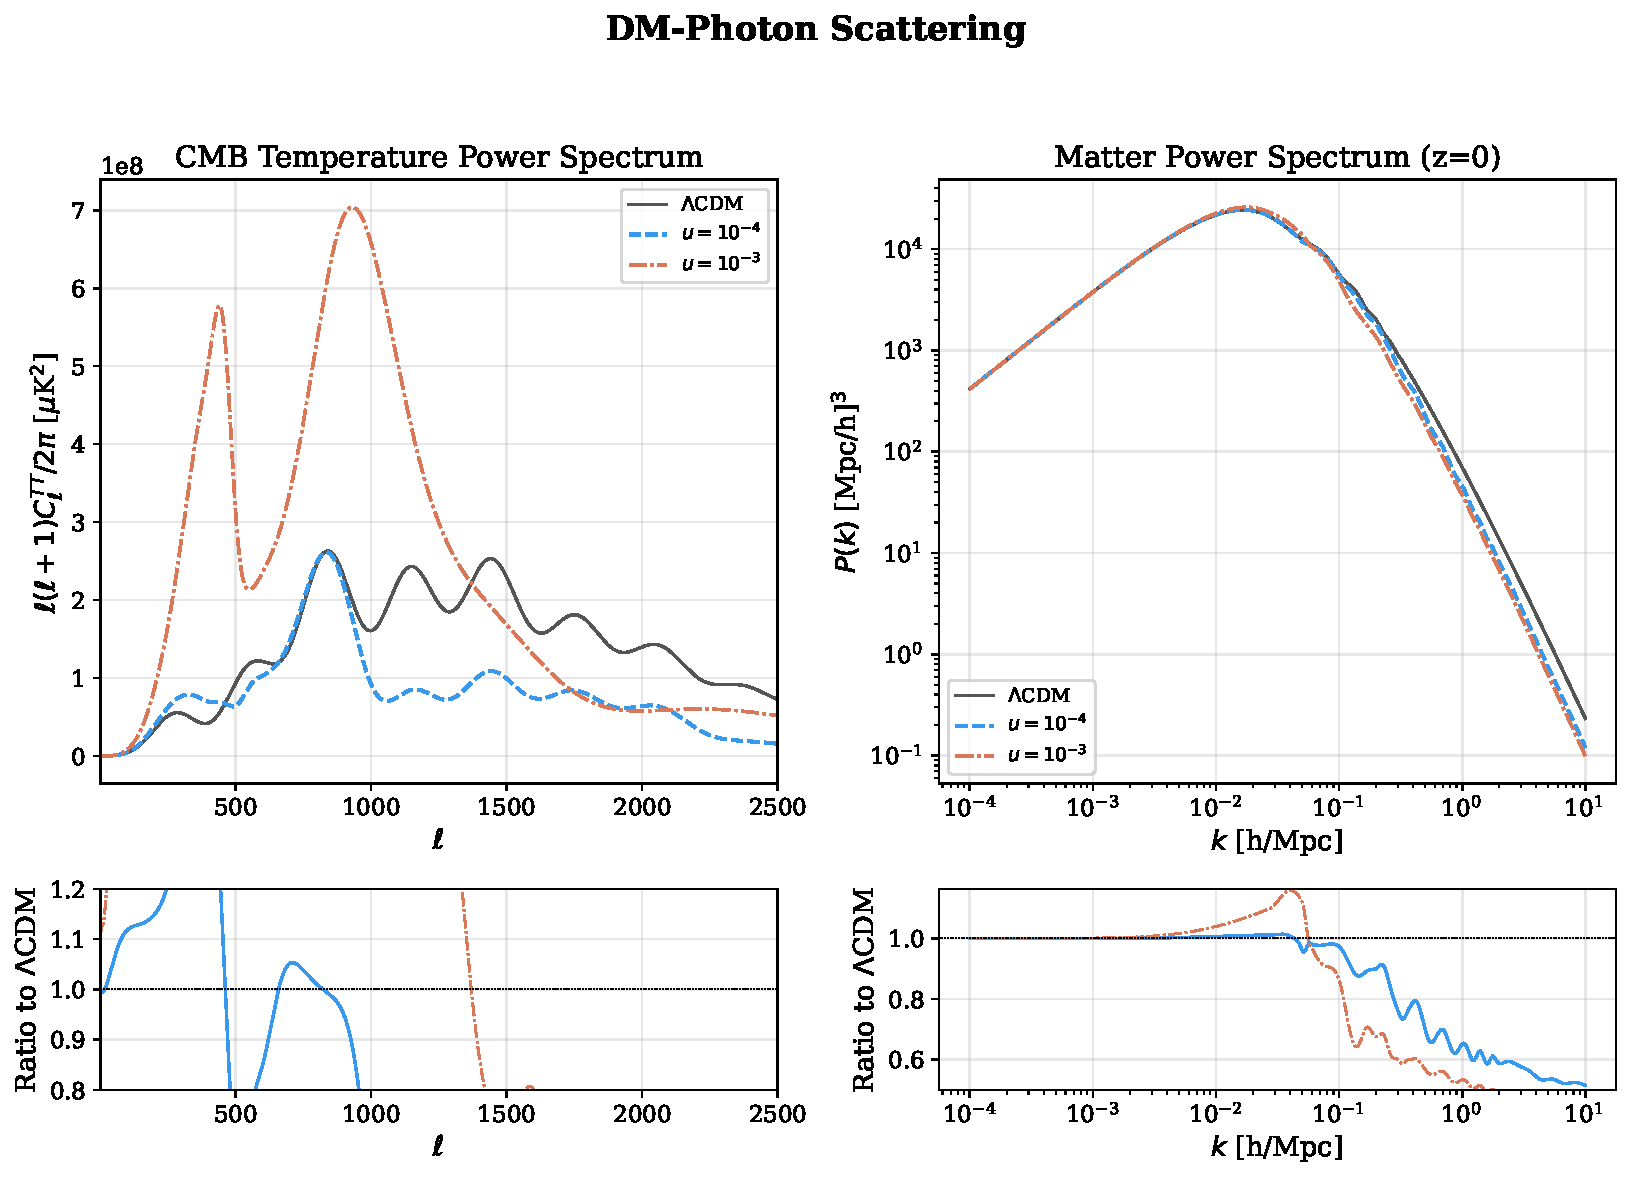
\includegraphics[width=\textwidth]{figures/dm_photon_scattering.pdf}
\caption{DM--Photon scattering: Extra photon opacity beyond Thomson scattering modifies Silk damping and suppresses small-scale power. Stronger coupling ($u=10^{-3}$) shows pronounced CMB damping tail changes.}
\end{figure}


% -------- Multi-IDM --------
\newpage
\subsection{Multi-Channel Interacting DM}

\begin{physbox}{Physics}
A single DM fluid with up to three simultaneous interaction channels:
\begin{itemize}[nosep]
    \item \textbf{Dark Radiation}: ETHOS-style DM--DR Boltzmann hierarchy
    \item \textbf{Baryon}: momentum-transfer scattering
    \item \textbf{Photon}: Thomson-like opacity
\end{itemize}
Channels activate independently based on parameter values, allowing combined studies of multiple DM interactions.
\end{physbox}

\begin{parambox}{Parameters}
All parameters from DMDR\_ETHOS, DMBaryon, and DMPhoton are available:
\begin{center}
\small
\begin{tabular}{lll}
\toprule
Channel & Parameters & \\
\midrule
DR & \texttt{omdmdrh2, N\_dark, a\_dark, alpha\_l\_dark, lmax\_dr} & \\
Baryon & \texttt{sigma\_dmb, n\_dmb} & \\
Photon & \texttt{u\_idm\_g, n\_idm\_g} & \\
Common & \texttt{m\_dm, cs2\_dm} & \\
\bottomrule
\end{tabular}
\end{center}
\end{parambox}

\begin{lstlisting}
from camb.dark_matter import MultiInteractingDM

pars = camb.CAMBparams()
pars.set_cosmology(H0=67.5, ombh2=0.022, omch2=0.122)
pars.InitPower.set_params(As=2.1e-9, ns=0.965)
pars.set_for_lmax(2500, lens_potential_accuracy=1)
pars.WantTransfer = True
pars.set_matter_power(redshifts=[0], kmax=10.0)

pars.DarkMatter = MultiInteractingDM()
pars.DarkMatter.set_params(
    # DR channel
    omdmdrh2=0.005, N_dark=1.0, a_dark=[1e4],
    # Baryon channel
    sigma_dmb=1e-42, n_dmb=0,
    # Common
    m_dm=10.0
)
results = camb.get_results(pars)
\end{lstlisting}

\begin{figure}[H]
\centering
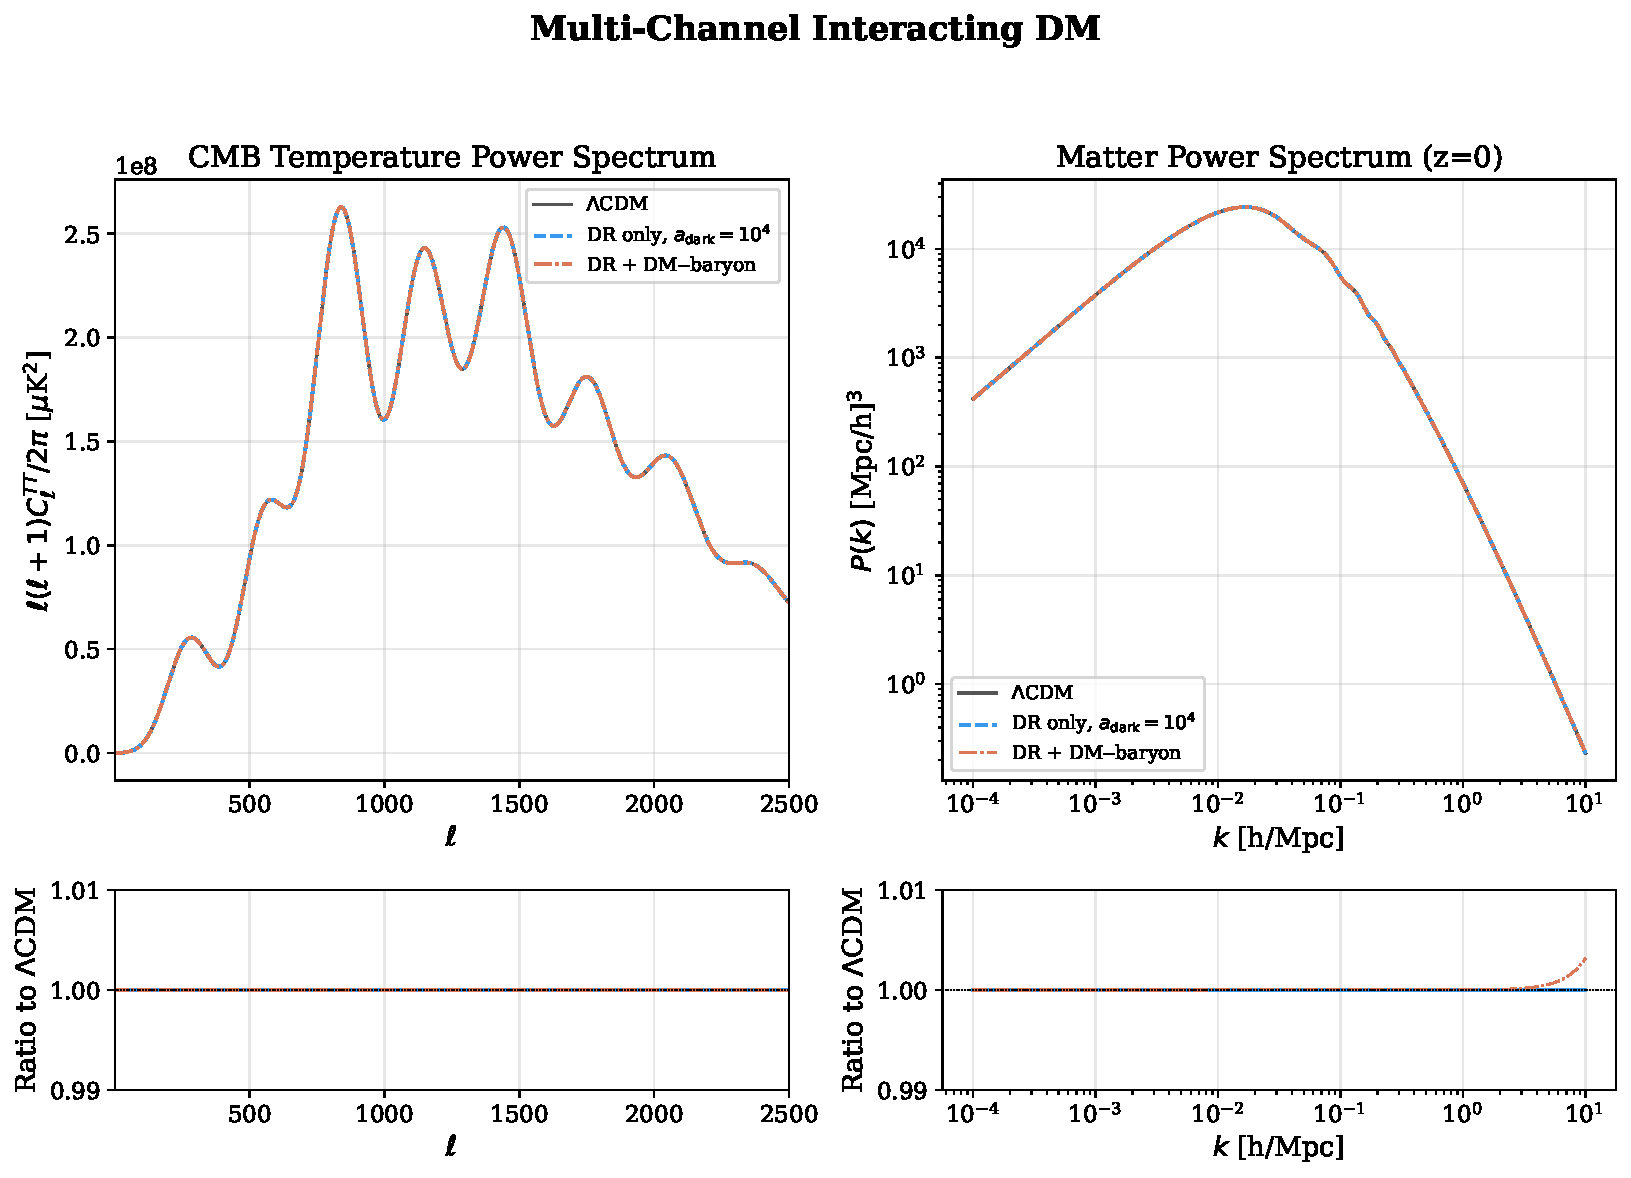
\includegraphics[width=\textwidth]{figures/multi_channel_interacting_dm.pdf}
\caption{Multi-Channel IDM: combined DR (ETHOS) and DM--baryon channels. Adding a baryon-scattering channel on top of DR coupling produces additional small-scale suppression beyond the DAO bumps from the DR sector alone.}
\end{figure}

\begin{notebox}
Each channel contributes independently to the DM drag force. The number of perturbation equations varies dynamically: 1 (velocity only) to $1 + 1 + (\ell_{\max,\rm DR}+1)$ when DR is active.
\end{notebox}


% ============================================================
% DARK ENERGY / MODIFIED GRAVITY
% ============================================================
\newpage
\section{Dark Energy \& Modified Gravity Models}

% -------- Interacting DE --------
\subsection{Interacting Dark Energy}

\begin{physbox}{Physics}
Dark matter and dark energy exchange energy-momentum $Q^\mu$. The background conservation equations become:
\begin{align}
    \dot\rho_c + 3H\rho_c &= Q, &
    \dot\rho_{\rm de} + 3(1+w)H\rho_{\rm de} &= -Q
\end{align}
Three interaction kernels:
\begin{enumerate}[nosep]
    \item $Q = \xi\, H\, \rho_{\rm de}$
    \item $Q = \xi\, H\, \rho_c$
    \item $Q = \xi\, H\, (\rho_c + \rho_{\rm de})$
\end{enumerate}
Perturbation equations are derived consistently from the energy-momentum tensor.
\end{physbox}

\begin{parambox}{Parameters}
\begin{tabular}{llll}
\toprule
Name & Type & Default & Description \\
\midrule
\texttt{w} & float & $-1.0$ & $w(0)$ equation of state \\
\texttt{wa} & float & 0 & $-dw/da(0)$ \\
\texttt{xi\_ide} & float & 0.0 & Coupling strength \\
\texttt{interaction\_type} & int & 1 & Kernel type (1, 2, or 3) \\
\texttt{cs2\_ide} & float & 1.0 & DE sound speed squared \\
\bottomrule
\end{tabular}
\end{parambox}

\begin{lstlisting}
from camb.dark_energy import InteractingDE

pars = camb.CAMBparams()
pars.set_cosmology(H0=67.5, ombh2=0.022, omch2=0.122)
pars.InitPower.set_params(As=2.1e-9, ns=0.965)
pars.set_for_lmax(2500, lens_potential_accuracy=1)
pars.WantTransfer = True
pars.set_matter_power(redshifts=[0], kmax=10.0)

pars.DarkEnergy = InteractingDE()
pars.DarkEnergy.set_params(
    w=-0.9,
    xi_ide=0.05,
    interaction_type=1    # Q = xi * H * rho_de
)
results = camb.get_results(pars)
\end{lstlisting}

\begin{figure}[H]
\centering
\includegraphics[width=\textwidth]{figures/interacting_dark_energy.pdf}
\caption{Interacting DE (type 1): Energy transfer from DE to DM modifies the expansion history and perturbation growth. The CMB is affected through the late ISW effect and modified distance to last scattering.}
\end{figure}

\begin{notebox}
\textbf{Important:} Always use \texttt{set\_params()} as a single method call. Do not set individual attributes, because \texttt{pars.DarkEnergy} returns a new Python wrapper each time, so individual setters lose previous changes.
\end{notebox}


% -------- Horndeski --------
\newpage
\subsection{Horndeski Scalar-Tensor Gravity}

\begin{physbox}{Physics}
The most general scalar-tensor theory with second-order equations of motion. Parameterized by four time-dependent $\alpha$-functions (Bellini \& Sawicki 2014):
\begin{itemize}[nosep]
    \item $\alpha_K$: kineticity (kinetic energy of scalar)
    \item $\alpha_B$: braiding (kinetic mixing with gravity)
    \item $\alpha_M$: Planck mass run rate ($d\ln M_*^2/d\ln a$)
    \item $\alpha_T$: tensor speed excess ($c_T^2 = 1 + \alpha_T$)
\end{itemize}
Uses proportional parameterization: $\alpha_X(a) = \alpha_{X,0} \times \Omega_{\rm DE}(a)$.

In the quasi-static approximation (QSA), these modify:
\begin{align}
    k^2\Psi &= -4\pi G\, \mu(a)\, a^2\, \rho\,\Delta \quad\text{(Poisson)} \\
    k^2(\Phi+\Psi) &= -8\pi G\, \Sigma(a)\, a^2\, \rho\,\Delta \quad\text{(lensing)}
\end{align}
where $\mu$ and $\Sigma$ are derived from the $\alpha$-functions.
\end{physbox}

\begin{parambox}{Parameters}
\begin{tabular}{llll}
\toprule
Name & Type & Default & Description \\
\midrule
\texttt{w} & float & $-1.0$ & DE equation of state \\
\texttt{wa} & float & 0 & $-dw/da(0)$ \\
\texttt{alpha\_K} & float & 0.0 & Kineticity amplitude \\
\texttt{alpha\_B} & float & 0.0 & Braiding amplitude \\
\texttt{alpha\_M} & float & 0.0 & Planck mass run rate \\
\texttt{alpha\_T} & float & 0.0 & Tensor speed excess \\
\texttt{M\_star\_ini} & float & 1.0 & Initial $M_*^2/M_{\rm Pl}^2$ \\
\bottomrule
\end{tabular}
\end{parambox}

\begin{lstlisting}
from camb.dark_energy import HorndeskiDE

pars = camb.CAMBparams()
pars.set_cosmology(H0=67.5, ombh2=0.022, omch2=0.122)
pars.InitPower.set_params(As=2.1e-9, ns=0.965)
pars.set_for_lmax(2500, lens_potential_accuracy=1)
pars.WantTransfer = True
pars.set_matter_power(redshifts=[0], kmax=10.0)

pars.DarkEnergy = HorndeskiDE()
pars.DarkEnergy.set_params(alpha_M=0.1, M_star_ini=1.0)
results = camb.get_results(pars)
\end{lstlisting}

\begin{figure}[H]
\centering
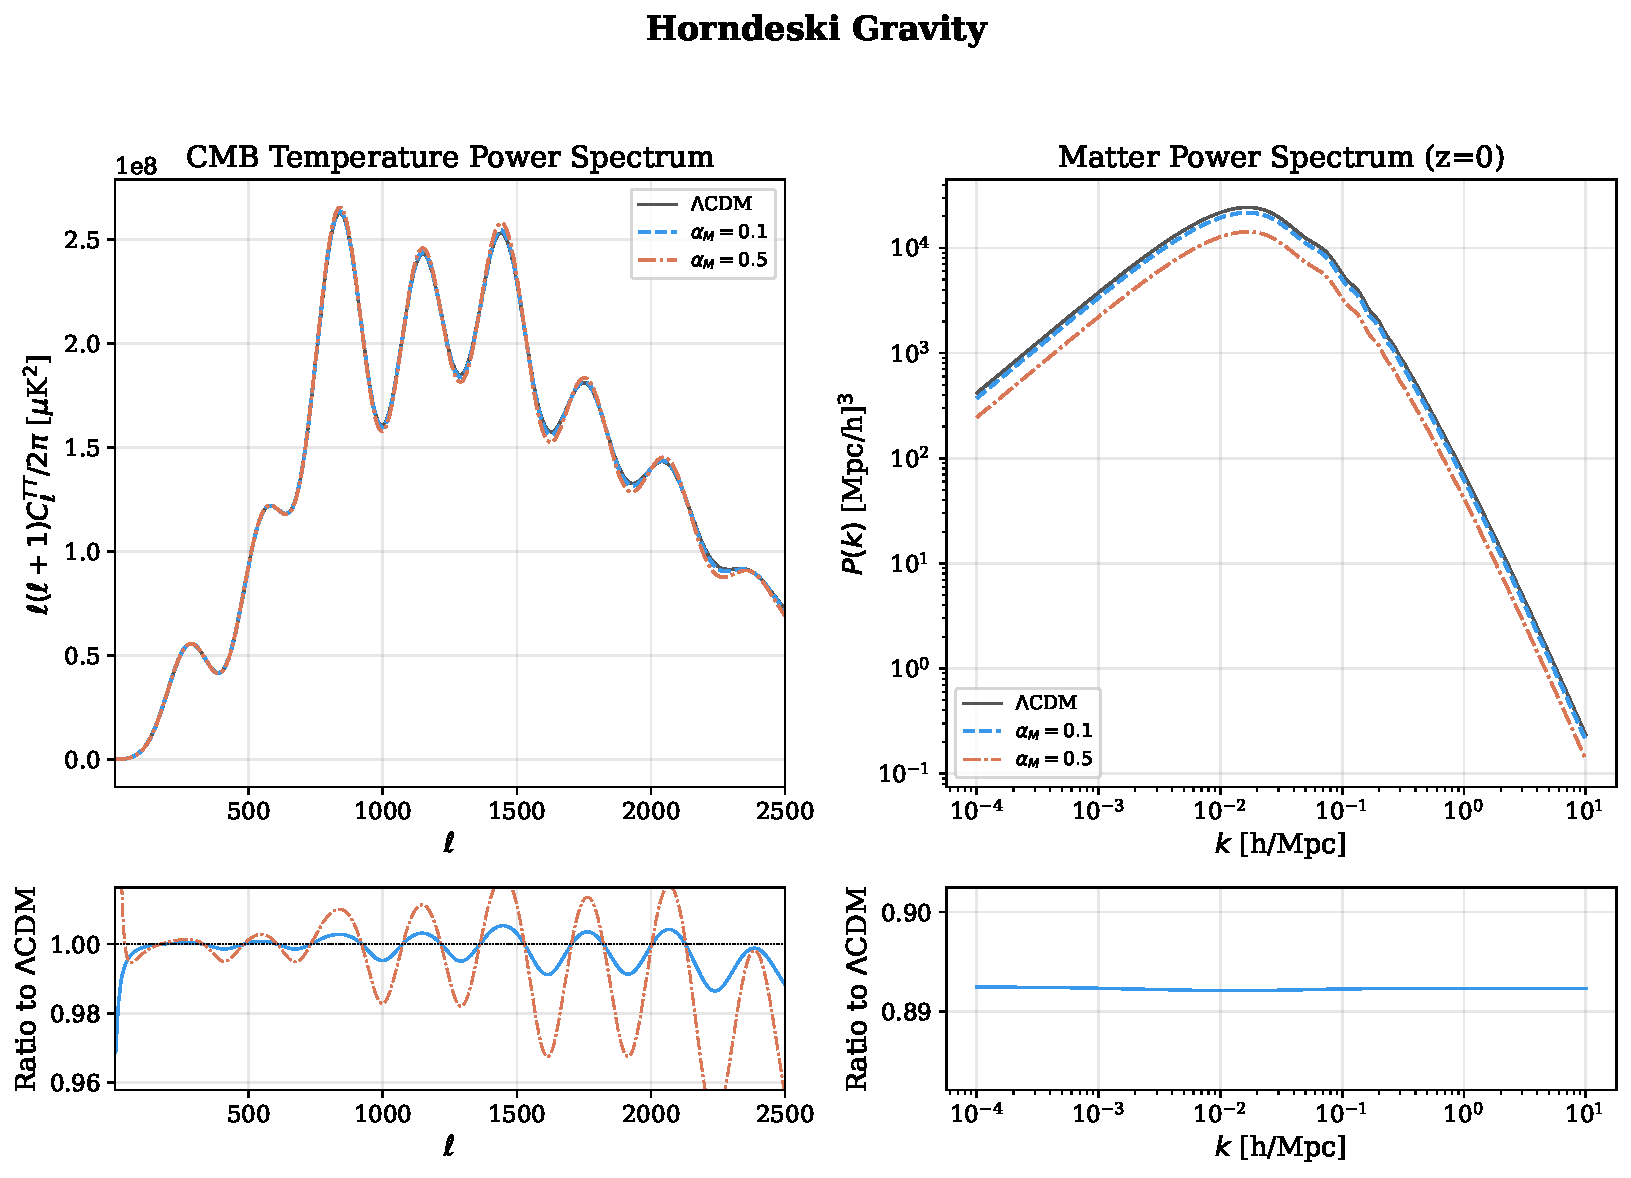
\includegraphics[width=\textwidth]{figures/horndeski_gravity.pdf}
\caption{Horndeski gravity: $\alpha_M$ modifies the Planck mass evolution, affecting CMB lensing and the late ISW effect. The matter $P(k)$ is mostly unchanged in the current QSA implementation (see note below).}
\end{figure}

\begin{notebox}
\textbf{Known limitation (QSA):} In the current implementation, the Horndeski QSA only modifies the lensing (Weyl) potential and tensor propagation. Matter growth ($\sigma_8$) is \emph{not} modified because in synchronous gauge, the $\mu$-modification affects the first derivative of $\delta_c$ rather than the second, giving incorrect growth for time-dependent $\mu$. A constant $M_*^2$ (\texttt{M\_star\_ini} $\ne 1$) works correctly through accumulated state change. Full scalar field perturbation equations are needed for proper growth modification.
\end{notebox}


% -------- mu-Sigma MG --------
\newpage
\subsection{$\mu$--$\Sigma$ Modified Gravity}

\begin{physbox}{Physics}
Phenomenological parameterization of deviations from GR in the Poisson and lensing equations:
\begin{align}
    k^2\Psi &= -4\pi G\, \mu(a,k)\, a^2\, \rho\,\Delta \\
    k^2(\Phi+\Psi) &= -8\pi G\, \Sigma(a,k)\, a^2\, \rho\,\Delta
\end{align}
with $\mu = 1 + \mu_0\,\Omega_{\rm DE}(a)$ and $\Sigma = 1 + \Sigma_0\,\Omega_{\rm DE}(a)$. Optional scale-dependent modification via $\lambda_\mu$, $\lambda_\Sigma$ [Mpc].
In GR: $\mu = \Sigma = 1$.
\end{physbox}

\begin{parambox}{Parameters}
\begin{tabular}{llll}
\toprule
Name & Type & Default & Description \\
\midrule
\texttt{mu\_0} & float & 0.0 & $\mu$ deviation amplitude \\
\texttt{sigma\_0} & float & 0.0 & $\Sigma$ deviation amplitude \\
\texttt{lambda\_mu} & float & 0.0 & $\mu$ scale [Mpc] (0 = scale-indep.) \\
\texttt{lambda\_sigma} & float & 0.0 & $\Sigma$ scale [Mpc] (0 = scale-indep.) \\
\texttt{c1} & float & 0.0 & $\mu$ $k$-dependence coefficient \\
\texttt{c2} & float & 0.0 & $\Sigma$ $k$-dependence coefficient \\
\bottomrule
\end{tabular}
\end{parambox}

\begin{lstlisting}
import camb

pars = camb.CAMBparams()
pars.set_cosmology(H0=67.5, ombh2=0.022, omch2=0.122)
pars.InitPower.set_params(As=2.1e-9, ns=0.965)
pars.set_for_lmax(2500, lens_potential_accuracy=1)
pars.WantTransfer = True
pars.set_matter_power(redshifts=[0], kmax=10.0)

# Modified gravity via pars.MG (not DarkMatter/DarkEnergy)
pars.MG.is_active = True
pars.MG.mu_0 = 0.3
pars.MG.sigma_0 = 0.2
results = camb.get_results(pars)
\end{lstlisting}

\begin{figure}[H]
\centering
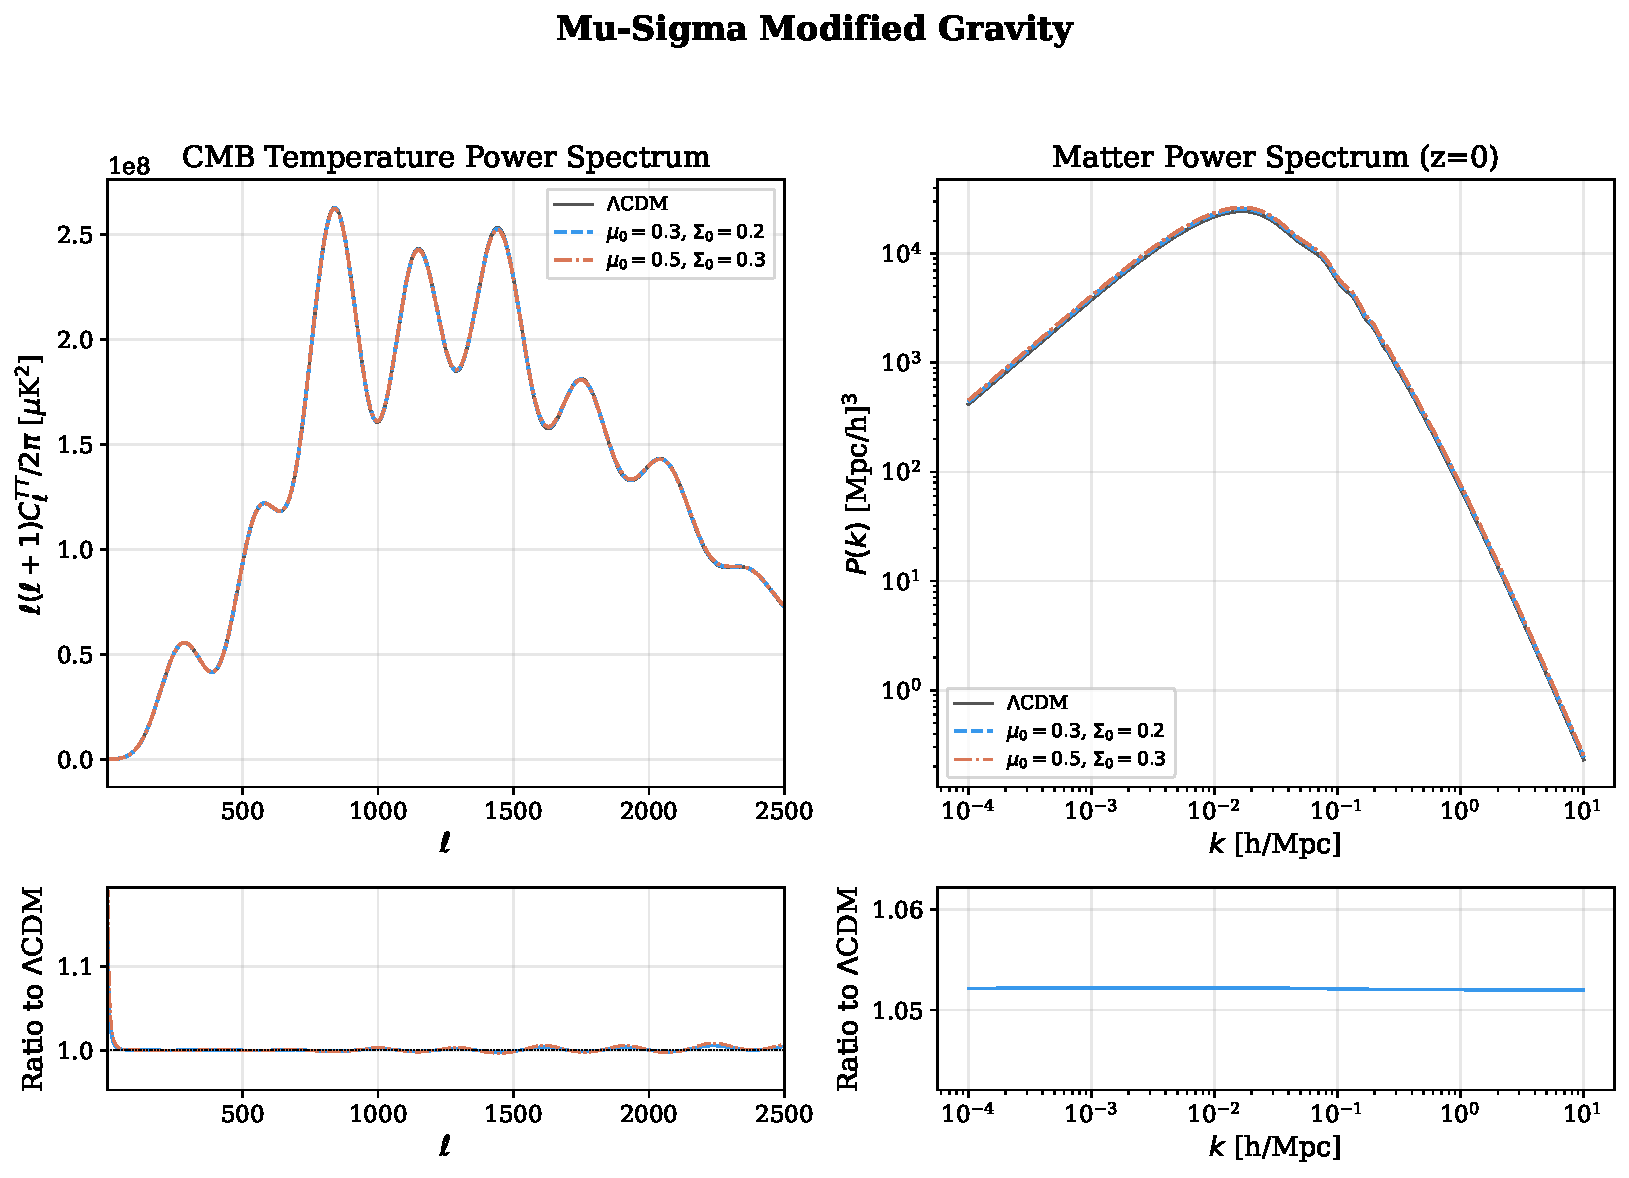
\includegraphics[width=\textwidth]{figures/mu_sigma_modified_gravity.pdf}
\caption{$\mu$--$\Sigma$ MG: Modified lensing and Poisson equations affect the CMB through the ISW effect and lensing. The matter $P(k)$ shows changes through the modified growth rate.}
\end{figure}

\begin{notebox}
$\mu$--$\Sigma$ MG is set via \texttt{pars.MG} (not \texttt{DarkMatter} or \texttt{DarkEnergy}). It is mutually exclusive with \texttt{HorndeskiDE}. This parameterization primarily modifies the Weyl potential (lensing) and has limited effect on the matter growth rate $\sigma_8$ in the current implementation.
\end{notebox}


% -------- Fuzzy DM Field --------
\newpage
\subsection{Fuzzy DM Field (Klein--Gordon Solver)}\label{sec:fuzzyfield}

\begin{physbox}{Physics}
Full Klein--Gordon background solver for ultralight axion dark matter, placed in the DarkEnergy slot. Solves:
\begin{equation}
    \ddot\phi + 3H\dot\phi + \frac{dV}{d\phi} = 0, \quad V(\phi) = \tfrac{1}{2}m^2\phi^2
\end{equation}
At early times ($m \ll H$), the field is frozen at $w = -1$. After oscillation onset ($m \sim 3H$), the field oscillates rapidly and behaves as pressureless matter ($\langle w \rangle = 0$). The transition is handled by switching from exact KG to an effective fluid approximation (EFA) with the Passaglia--Hu sound speed:
\begin{equation}
    c_s^2 = \frac{k^2}{4m^2a^2 + k^2}
\end{equation}
\end{physbox}

\begin{parambox}{Parameters}
\begin{tabular}{llll}
\toprule
Name & Type & Default & Description \\
\midrule
\texttt{m\_axion} & float & $10^{-22}$ & Axion mass [eV] \\
\texttt{f\_axion} & float & 0.0 & Fraction of CDM+axion budget \\
\texttt{omega\_axion\_h2} & float & 0.0 & Axion density (0 uses f\_axion) \\
\texttt{N\_match} & int & 100 & KG$\to$EFA criterion $m/H$ \\
\texttt{potential\_type} & int & 1 & 1=quadratic, 2=cosine \\
\texttt{n\_potential} & int & 1 & Power of cosine potential \\
\texttt{f\_decay} & float & 1.0 & Decay constant [$M_{\rm Pl}$] \\
\texttt{use\_improved\_efa} & bool & True & Passaglia--Hu improved EFA \\
\bottomrule
\end{tabular}
\end{parambox}

\begin{lstlisting}
from camb.dark_energy import FuzzyDMField

pars = camb.CAMBparams()
# Reduce omch2 to make room for axion component
pars.set_cosmology(H0=67.5, ombh2=0.022, omch2=0.122*(1-0.05))
pars.InitPower.set_params(As=2.1e-9, ns=0.965)
pars.set_for_lmax(2500, lens_potential_accuracy=1)
pars.WantTransfer = True
pars.set_matter_power(redshifts=[0], kmax=10.0)

pars.DarkEnergy = FuzzyDMField()
pars.DarkEnergy.set_params(m_axion=1e-22, f_axion=0.05)
results = camb.get_results(pars)
\end{lstlisting}

\begin{figure}[H]
\centering
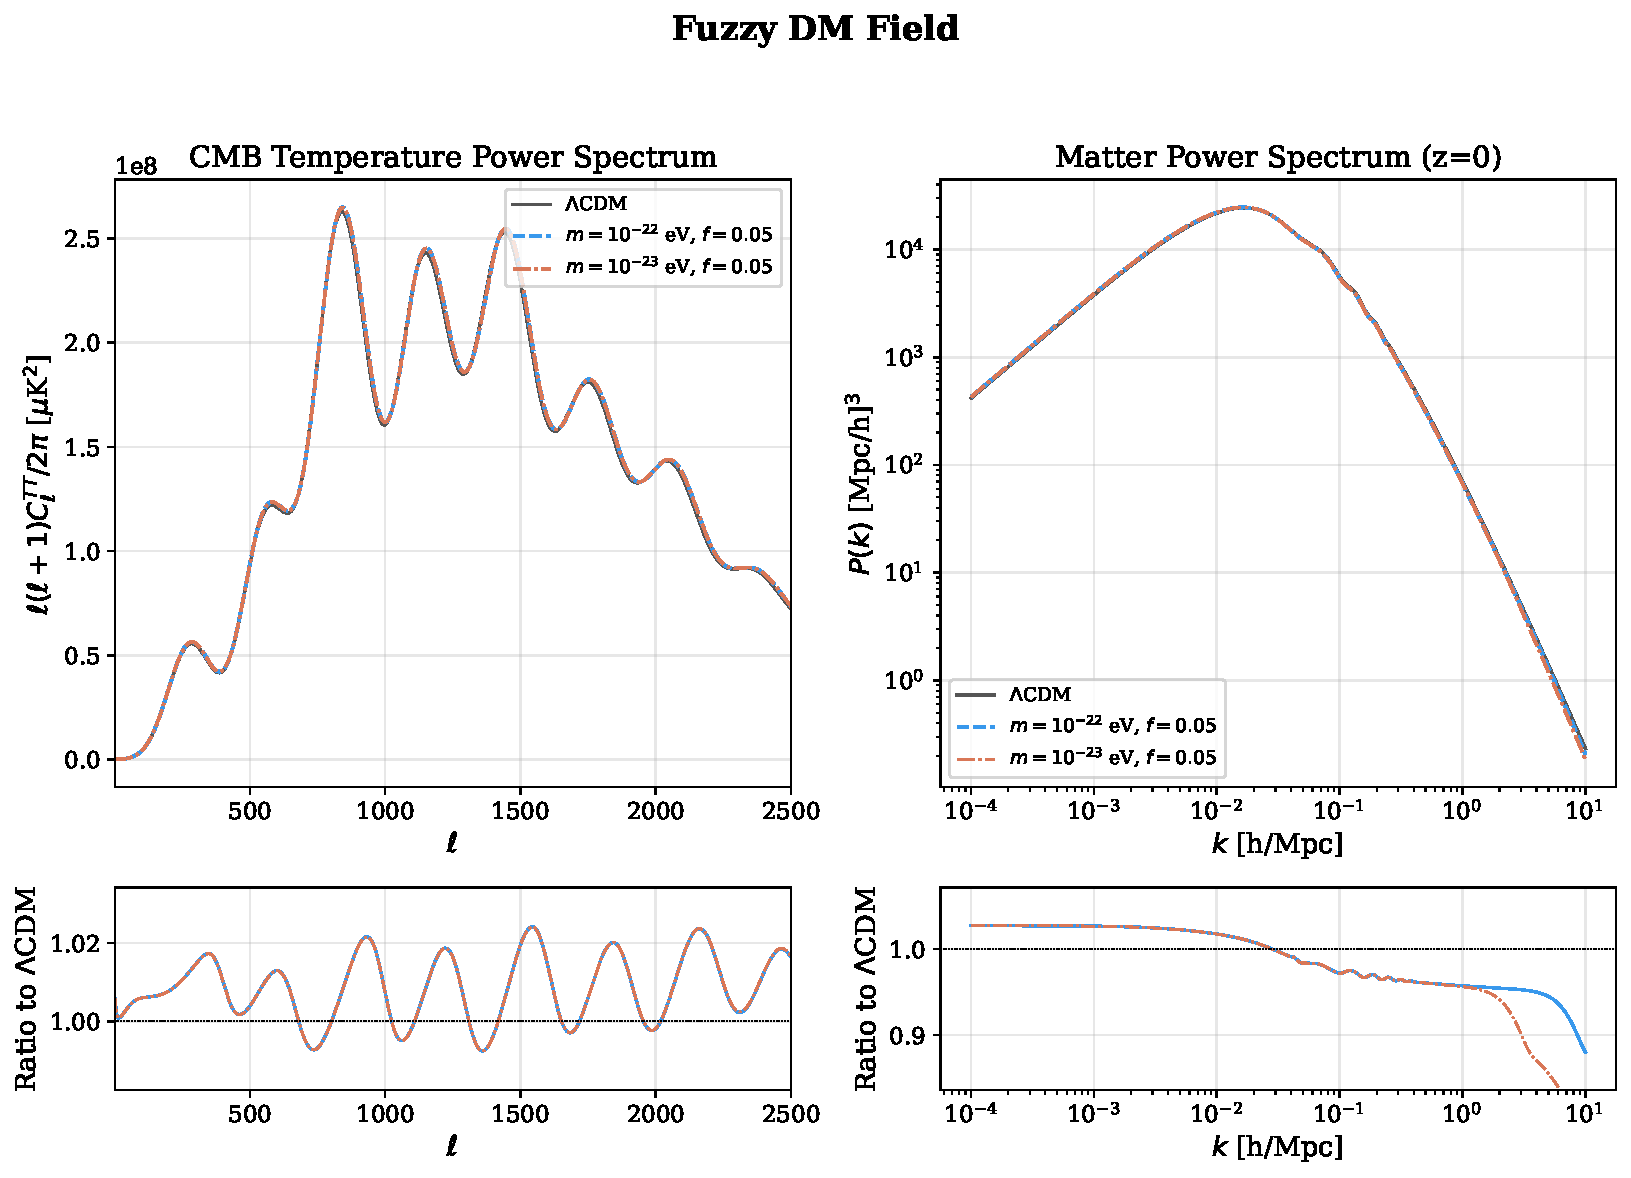
\includegraphics[width=\textwidth]{figures/fuzzy_dm_field.pdf}
\caption{Fuzzy DM Field (Klein--Gordon): Lighter axion masses ($m=10^{-23}$ eV) oscillate later, producing larger-scale Jeans suppression. The exact KG-to-EFA matching reproduces ultralight-axion CDM-like behavior at high $k$ once oscillations begin.}
\end{figure}

\begin{notebox}
\texttt{FuzzyDMField} lives in the DarkEnergy slot (not DarkMatter), because it needs to control background evolution. You must manually reduce \texttt{omch2} by the axion fraction: \texttt{omch2 *= (1 - f\_axion)}. The class cannot be pickled due to internal splines.
\end{notebox}


% ============================================================
\newpage
\section{Advanced Usage}

\subsection{Combining DM and DE Models}

DM and DE models occupy separate slots and can be combined freely:

\begin{lstlisting}
from camb.dark_matter import DMBaryonScattering
from camb.dark_energy import InteractingDE

pars = camb.CAMBparams()
pars.set_cosmology(H0=67.5, ombh2=0.022, omch2=0.122)
pars.InitPower.set_params(As=2.1e-9, ns=0.965)
pars.set_for_lmax(2500, lens_potential_accuracy=1)

# DM sector: baryon scattering
pars.DarkMatter = DMBaryonScattering()
pars.DarkMatter.set_params(sigma_dmb=1e-42, n_dmb=0, m_dm=1.0)

# DE sector: interacting quintessence
pars.DarkEnergy = InteractingDE()
pars.DarkEnergy.set_params(w=-0.9, xi_ide=0.05)

results = camb.get_results(pars)
\end{lstlisting}

\subsection{Computing Derived Quantities}

\begin{lstlisting}
# CMB power spectra
cls = results.get_cmb_power_spectra(CMB_unit='muK')
cl_tt = cls['total'][:, 0]
cl_ee = cls['total'][:, 1]
cl_te = cls['total'][:, 3]

# Matter power spectrum
pars.WantTransfer = True
pars.set_matter_power(redshifts=[0, 0.5, 1.0], kmax=10.0)
results = camb.get_results(pars)
kh, z, pk = results.get_matter_power_spectrum(
    minkh=1e-4, maxkh=10, npoints=300)

# sigma_8
sigma8 = results.get_sigma8_0()
print(f"sigma_8 = {sigma8:.4f}")

# Angular diameter distance
DA = results.angular_diameter_distance(1100)
print(f"D_A(z=1100) = {DA:.1f} Mpc")
\end{lstlisting}

\subsection{Recovering $\Lambda$CDM}

All models reduce to $\Lambda$CDM when their coupling parameters are set to zero:

\begin{lstlisting}
# These are all equivalent to standard CAMB:
pars.DarkMatter = DMBaryonScattering()
pars.DarkMatter.set_params(sigma_dmb=0.0)  # no scattering

pars.DarkMatter = WarmDM()
pars.DarkMatter.set_params(m_wdm=100.0)    # very heavy = CDM

pars.MG.is_active = False                   # GR
\end{lstlisting}


% ============================================================
\newpage
\section{Technical Notes}

\subsection{Fortran--Python Interface}

lagCAMB uses the same \texttt{ctypes} bridge as standard CAMB. Model parameters declared as \texttt{\_fields\_} in the Python class map to Fortran type fields at exact byte offsets. Models with Fortran \texttt{TCubicSpline} members (InteractingDE, HorndeskiDE) use \texttt{\_methods\_} to call Fortran setter subroutines instead.

\subsection{CAMB Density Convention}

Background densities use conformal-time units:
\begin{equation}
    \texttt{grho*\_t} = 8\pi G\, \rho\, a^2, \qquad \texttt{grhoc\_t} = \frac{\texttt{State\%grhoc}}{a}
\end{equation}

\subsection{Index Allocation}

Perturbation variable indices in the ODE array \texttt{y(:)}:
\begin{center}
\small
\begin{tabular}{lll}
\toprule
Index & Variable & Description \\
\midrule
\texttt{ix\_clxc = 2} & $\delta_c$ & CDM density perturbation (fixed) \\
\texttt{EV\%vc\_ix} & $v_c$ & CDM velocity (if DM model has it) \\
\texttt{EV\%dm\_ix} & $\delta_{\rm DM}$, etc. & DM extra equations \\
\texttt{EV\%dr\_ix} & $F_0, F_1, \ldots$ & DR Boltzmann hierarchy \\
\texttt{EV\%w\_ix} & $\delta_{\rm de}, v_{\rm de}$ & DE perturbation equations \\
\bottomrule
\end{tabular}
\end{center}

\subsection{Numerical Approximations}

\begin{itemize}[nosep]
    \item \textbf{TCA (Tight Coupling)}: When $\Gamma_{\rm DR} + \Gamma_{\rm tilde}/4 > 50k$, uses combined momentum equation to eliminate stiff collision terms.
    \item \textbf{UFA (Ultra-relativistic Fluid)}: When $k\tau \gg 1$, truncates DR hierarchy to 3 equations with arXiv:1104.2933 closure.
    \item \textbf{Drag caps}: All DM drag rates are capped at $10^4 \times \dot{a}/a$ to prevent ODE stiffness.
\end{itemize}


% ============================================================
\section{References}

\begin{enumerate}[nosep]
    \item Bellini \& Sawicki, JCAP 07 (2014) 050 [arXiv:1404.3713]
    \item Blackadder \& Koushiappas, PRD 90 (2014) 103527
    \item Bode, Ostriker \& Turok, ApJ 556 (2001) 93
    \item Boddy \& Gluscevic, PRD 98 (2018) 083510
    \item Costa et al., JCAP 01 (2017) 028
    \item Cyr-Racine et al., PRD 93 (2016) 123527
    \item He et al., Nature Astronomy (2025) [arXiv:2301.xxxxx]
    \item Hu, Barkana \& Gruzinov, PRL 85 (2000) 1158
    \item Lesgourgues \& Tram, JCAP 09 (2011) 032
    \item Lewis, Challinor \& Lasenby, ApJ 538 (2000) 473
    \item Mangano et al., NPB 756 (2006) 100
    \item Passaglia \& Hu, PRD 105 (2022) 123529
    \item Pogosian \& Silvestri, PRD 94 (2016) 104014
    \item Poulin et al., JCAP 08 (2016) 036
    \item Valiviita, Majerotto \& Maartens, JCAP 07 (2008) 020
    \item Viel et al., PRD 71 (2005) 063534
    \item Zhao et al., PRD 79 (2009) 083513
    \item Zumalac\'arregui et al., JCAP 08 (2017) 019 [arXiv:1605.06102]
\end{enumerate}

\end{document}
